\section{Separation of Signal from Background Using Matrix Elements}
\label{separation-ME}

\subsection{Method Overiew}
\subsection{Calculation of the Event Probability Density Functions}
\subsubsection{Differential Cross Section}
\subsubsection{Cross Section}
\subsubsection{Treatment of Combinatorial Background}
\subsection{Single Top Discriminant}
\subsubsection{One-Dimensional Discriminants}
\subsubsection{Performance}
\subsubsection{Two-Dimensional Discrimiannts}


\subsection{Method Description}
The matrix element analysis uses leading order matrix elements to separate
single top quark events from background events. The matrix
element analysis calculates the probability for an event to be a signal top event,
either $s$-channel or $t$-channel, and a probability for one of several $W$+jets
backgrounds. This probability is defined in Eq.~\ref{prob} as

\begin{equation}
\label{prob}
P(\vec{x}) = \frac{1}{\sigma} \sum_{i,j} \int f_{i}(q_{1}, Q^{2})dq_{1}
\times 
f_{j}(q_{2}, Q^{2})dq_{2} \times \pderiv{\sigma_{hs,ij}(\vec{y})}{\vec{y}}
\times W(\vec{x},\vec{y})d\vec{y}
\end{equation}

\noindent Each term in the Eq.~\ref{prob} is described below.

\begin{itemize}
\item $\sum_{i,j}$ is a sum of initial parton flavors in the hard scatter
collision. For example, an $s$-channel collision can occur from a $u\bar{d}$,
$c\bar{s}$, $d\bar{u}$, or $s\bar{c}$.
\item $f_{i}(q_{1}, Q^{2})$ is the parton distribution function for parton, $i$.
\item $\pderiv{\sigma_{hs,ij}(\vec{y})}{\vec{y}}$ is the differential cross
section for the hard scatter collision.
\item $W(\vec{x},\vec{y})$ is called the transfer function which relates observed
objects in the detector, $\vec{x}$, to the final state objects from the matrix
element, $\vec{y}$.
\item $\int d\vec{y}$ is an integration over the matrix element phase space.
\item $\frac{1}{\sigma}$ is the normalization constant and is described in
Eq.~\ref{cross}.
\end{itemize}

\begin{equation}
\label{cross}
\sigma = \sum_{i,j} \int f_{i}(x_{1}, Q^{2})dx_{1}
\times 
f_{j}(x_{2}, Q^{2})dx_{2} \times \pderiv{\sigma_{hs,ij}(\vec{y})}{\vec{y}}
\times W(\vec{x},\vec{y})d\vec{y}d\vec{x} \times \varepsilon(\vec{x}) \times
\Theta_{\rm{cuts}}(\vec{x})
\end{equation}

\noindent This analysis uses CTEQ 6.1 LO~\cite{Pumplin:2005rh} parton distribution
functions access via LHAPDF~\cite{LHAPDF}. Matrix elements in
this analysis were taken from the Madgraph~\cite{Maltoni:2002qb} leading
order matrix element generator. The multidimensional integrals were calculated
using the GNU~\cite{GNU} Scientific Library's version of the VEGAS Monte Carlo integration technique ~\cite{Lepage:1980dq}.

The transfer functions, $W(\vec{x},\vec{y})$, relate the
observed state in the detector to the final state at the parton level. These
functions are determined using Monte Carlo where the final state flavor and
four-vector is known. A transfer function is determined for each jet flavor and
for several regions of the calorimeter. The functions used in this analysis as the same
as the ones used in the top mass analysis~\cite{JetTF}. An example plot of the
average energy difference between partons and jets for each jet flavor is shown
in Fig~\ref{FlavorTF}.

\vspace{0.1in}
\begin{figure}[!h!tbp]
\begin{center}
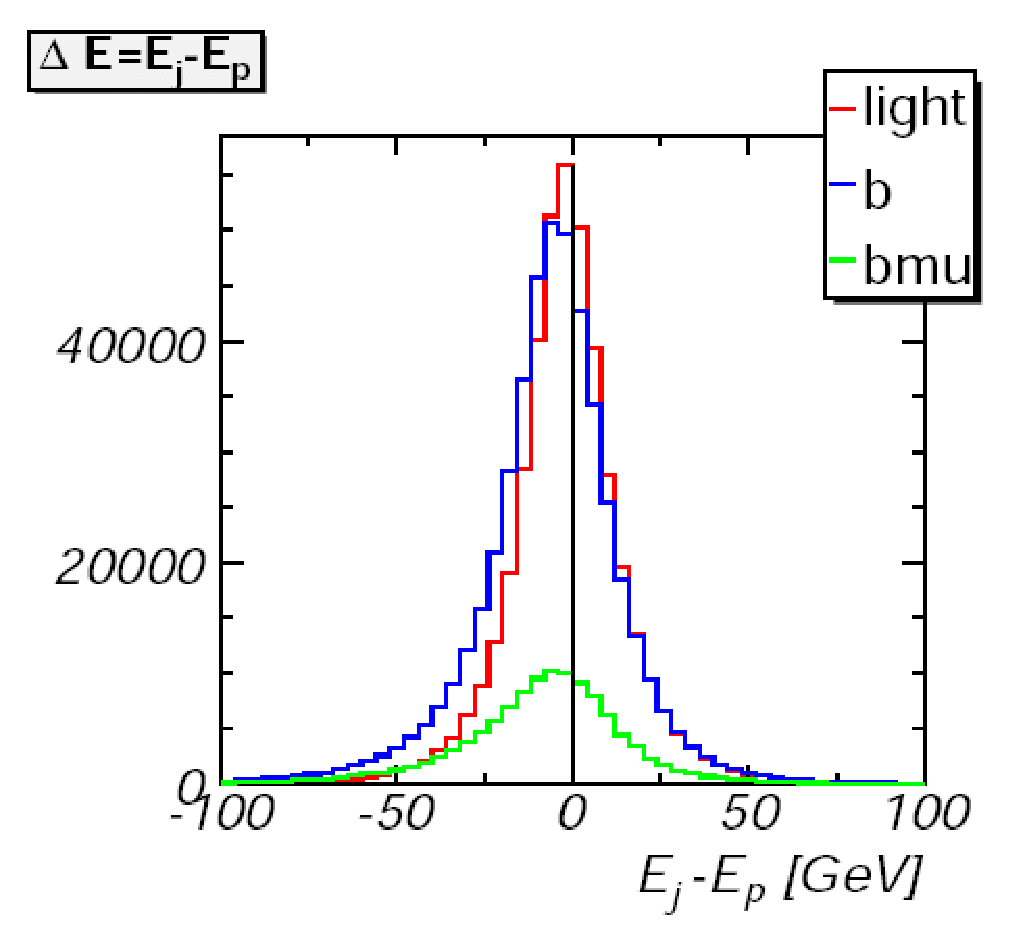
\includegraphics[width=0.48\textwidth]{figures/transfer/tfs.eps}
\end{center}
\vspace{-0.1in}
\caption[2jets]{Energy difference between a jet a match parton for three types
of jets.}
\label{FlavorTF}
\end{figure}

The muon transfer functions were determined for muons with and without
an SMT hit and are parametrized as a function of
$\large{\frac{1}{p_{T}}}$. The functions used in this analysis were
again the same as the ones used in the top mass
analysis~\cite{MuonTF,MuonTF2}. Lei Wang provided us the electron
resolution as a function of $\eta$ and $E$, out of which we made
Gaussian transfer functions.~\cite{ElectronTF}.

The event probabilities shown in Eq.~\ref{prob} assume a particle
assignment of a jet to a parton in the final state. In practice, this assignment
is not known and we must sum over all possible assignments to ensure the correct
one is chosen. This analysis uses
information from the neural network $b$ tagger to weight event where a b-Jet is
assigned to a $b$ quark and an untagged jet is assigned to a light flavor quark. The factor
$\varepsilon(\vec{x})$ is included in the probability calculation as the efficiency
for this $b$-tagging assignment. This efficiency is described in more detail in
appendix~\ref{JetPartonAssigmnent}. 

For two-jet events, the event probability is then re-written as a sum over
assignment possibilities as shown in Eq.~\ref{prob2jet}.

\begin{equation}
\label{prob2jet}
P(\ell, \nu, j_{1}, j_{2}) = P(\ell, \nu, \rm{j}_{1} \rightarrow p_{1}, j_{2}
\rightarrow p_{2}) + P(\ell, \nu, \rm{j}_{1} \rightarrow p_{2}, j_{2} \rightarrow p_{1})
\end{equation}

%\noindent and the new event
%probability for three-jet events is shown in Eq.~\ref{prob3jet}.
%\begin{eqnarray}
%\label{prob3jet}
%\nonumber
%P(\ell, \nu, j_{1}, j_{2}, j_{3}) = P(\ell, \nu, \rm{j}_{1} \rightarrow p_{1}, j_{2} \rightarrow p_{2}, j_{3} \rightarrow p_{3}) + P(\ell, \nu, \rm{j}_{1} \rightarrow p_{1}, j_{2} \rightarrow p_{3}, j_{3} \rightarrow p_{2}) + \\
%\nonumber
%P(\ell, \nu, \rm{j}_{1} \rightarrow p_{2}, j_{2} \rightarrow p_{1}, j_{3} \rightarrow p_{3}) + P(\ell, \nu, \rm{j}_{1} \rightarrow p_{2}, j_{2} \rightarrow p_{3}, j_{3} \rightarrow p_{1}) + \\
%P(\ell, \nu, \rm{j}_{1} \rightarrow p_{3}, j_{2} \rightarrow p_{2}, j_{3} \rightarrow p_{1}) + P(\ell, \nu, \rm{j}_{1} \rightarrow p_{3}, j_{2} \rightarrow p_{1}, j_{3} \rightarrow p_{2})
%\end{eqnarray}


\subsection{Matrix Elements}

The matrix element analysis is named so because the differential cross section for the hard scatter interaction is proportional to the leading order matrix element~\cite{PDG} as shown in Eq.~\ref{me}

\begin{equation}
\label{me}
d\sigma_{hs} = \frac{(2\pi)^4}{4} \frac{{|\cal M|}^{2}}{\sqrt{(q_{1}q_{2})^2 - m_{1}^2
m_{2}^2}} d\Phi_{n}(y)
\end{equation}

\noindent For this analysis, we calculate five probabilities for two-jet events and 
three probabilities for three-jet events. For two-jet events events, we
calculate the probability for $s$-channel single top ($u\bar{d}$ $\rightarrow$
$t\bar{b}$), $t$-channel single top ($ub$ $\rightarrow$ $td$), Wbb production
($u\bar{d}$ $\rightarrow$ $Wb\bar{b}$), Wcg production ($sg$ $\rightarrow$
$W\bar{c}g$), and Wgg production ($u\bar{d}$ $\rightarrow$ $Wgg$). The leading order diagrams for these channels are shown in Fig~\ref{2jets}.

\vspace{0.1in}
\begin{figure}[!h!tbp]
\begin{center}
\subfigure[]{
	\includegraphics[width=0.24\textwidth]{figures/feynman/tb.eps}
}
\subfigure[]{
	\includegraphics[width=0.24\textwidth]{figures/feynman/tq.eps}
}
\subfigure[]{
	\includegraphics[width=0.24\textwidth]{figures/feynman/wbb.eps}
}
\subfigure[]{
	\includegraphics[width=0.24\textwidth]{figures/feynman/wcg.eps}
}
\subfigure[]{
	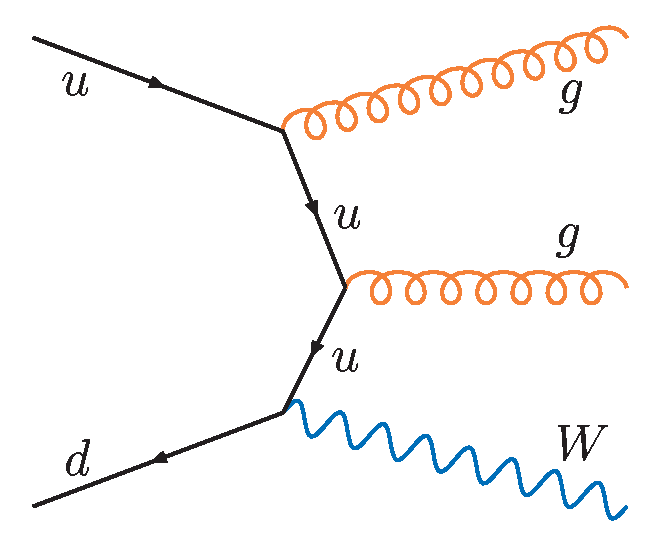
\includegraphics[width=0.24\textwidth]{figures/feynman/wgg.eps}
}
\end{center}
\vspace{-0.1in}
\caption[2jets]{The leading order matrix elements used for event probability
calculation for events with two jets. (a) $u\bar{d}$ $\rightarrow$ $t\bar{b}$,
(b) $ub$ $\rightarrow$ $td$, (c) $u\bar{d}$ $\rightarrow$ $Wb\bar{b}$, (d) $sg$
$\rightarrow$ $W\bar{c}g$, and (e) $u\bar{d}$ $\rightarrow$ $Wgg$}
\label{2jets}
\end{figure}

%For events with three jets, we use four matrix elements, $s$-channel with gluon
%radiation ($u\bar{d}$ $\rightarrow$ $t\bar{b}g$), $t$-channel with associated $b$
%quark ($ug$ $\rightarrow$ $t\bar{b}d$), Wbbg ($u\bar{d}$ $\rightarrow$
%$Wb\bar{b}g$), and Wugg ($g\bar{d}$ $\rightarrow$
%$W\bar{u}gg$. The leading order Feynman diagrams are shown in Fig~\ref{3jets}.

%\vspace{0.1in}
%\begin{figure}[!h!tbp]
%\begin{center}
%\subfigure[]{
%	\includegraphics[width=0.24\textwidth]{figures/feynman/tbg.eps}
%}
%\subfigure[]{
%	\includegraphics[width=0.24\textwidth]{figures/feynman/tqb.eps}
%}
%\subfigure[]{
%	\includegraphics[width=0.24\textwidth]{figures/feynman/wbbg.eps}
%}
%\subfigure[]{
%	\includegraphics[width=0.24\textwidth]{figures/feynman/wugg.eps}
%}
%\end{center}
%\vspace{-0.1in}
%\caption[3jets]{The leading order matrix elements used for event probability
%calculation for events with two jets.  (a) $u\bar{d}$ $\rightarrow$ $t\bar{b}g$,
%(b) $ug$ $\rightarrow$ $t\bar{b}d$, (c) $u\bar{d}$ $\rightarrow$ $Wb\bar{b}g$,
%and (d) $g\bar{d}$ $\rightarrow$ $W\bar{u}gg$}
%\label{3jets}
%\end{figure}

\subsection{Cross Sections}

To obtain a properly normalized probability density value for each event it is
necessary to calculate the signal or background cross section as defined in
Eq.~\ref{cross}. Summarized in table~\ref{crosssections} are the cross
sections used for each signal and background process.

All cross sections were calculated with these parton level cuts

\begin{itemize}
\item Parton Isolation: $\Delta$R($q_{i}$, $q_{j}$) $> 0.5$
\item Min Parton Energy: $q_{i}$ $P_{T}$ $> 6$ GeV
\item Max Parton Angle: $q_{i}$ $\eta <$ 3.5
\item No cuts were applied to the lepton or neutrino
\end{itemize}

and the following selection cuts on reconstructed objects

\begin{itemize}
\item Lepton $P_{T}$ $>$ 15.0 GeV
\item Electron(Muon) $|\eta|$ $<$ 1.1(2.0)
\item Missing $E_{T}$ $>$ 15.0 GeV
\item Leading Jet $P_{T}$ $>$ 25.0 GeV
\item Leading Jet $|\eta|$ $<$ 2.5
\item Second Jet $P_{T}$ $>$ 20.0 GeV
\item Second Jet $|\eta|$ $<$ 3.5
%\item Third Jet $P_{T}$ $>$ 20.0 GeV (if 3 jet event)
%\item Third Jet $|\eta|$ $<$ 3.5 (if 3 jet event)
\end{itemize}

All $W$+jets cross sections used $M_{W}^{2} + \sum_{jets}({M_{i}^2 + P_{i,T}^2})$ as
the factorization and renormalization scales while the single top cross sections
used $M_{\rm{top}}^{2}$. All cross sections have less than 1$\%$ error from the
Monte Carlo integration.

\vspace{0.05in}
\begin{table}[!h!tbp]
\begin{center}
\begin{minipage}{4.5 in}
\begin{ruledtabular}
\begin{tabular}{l||ccc}
\multicolumn{4}{c} {\hspace{0.5in}\underline{Cross Section $\times$ Branching Ratio For Each Source}}\vspace{0.1in} \\
Source					&	Lepton		&	Number of $b$ tags	&
	$\sigma \times B$ [fb]		\\
\hline
$p\bar{p}$ $\rightarrow$ $tq$		&	Electron	&	1	&
	19.6			\\
$p\bar{p}$ $\rightarrow$ $tq$		&	Electron	&	2	&
	0.27			\\
$p\bar{p}$ $\rightarrow$ $tq$		&	Muon	&	1	&
	26.8			\\
$p\bar{p}$ $\rightarrow$ $tq$		&	Muon	&	2	&
	0.38			\\
\hline
%$p\bar{p}$ $\rightarrow$ $tqb$		&	Electron	&	1	&
%	6.34			\\
%$p\bar{p}$ $\rightarrow$ $tqb$		&	Electron	&	2	&
%	5.40			\\
%$p\bar{p}$ $\rightarrow$ $tqb$		&	Muon	&	1	&
%	8.56			\\
%$p\bar{p}$ $\rightarrow$ $tqb$		&	Muon	&	2	&
%	7.40			\\
%\hline
$p\bar{p}$ $\rightarrow$ $t\bar{b}$	&	Electron	&	1	&
	8.07			\\
$p\bar{p}$ $\rightarrow$ $t\bar{b}$	&	Electron	&	2	&
	6.90			\\
$p\bar{p}$ $\rightarrow$ $t\bar{b}$	&	Muon	&	1	&
	10.4			\\
$p\bar{p}$ $\rightarrow$ $t\bar{b}$	&	Muon	&	2	&
	8.90			\\
\hline
%$p\bar{p}$ $\rightarrow$ $tbg$		&	Electron	&	1	&
%	6.02			\\
%$p\bar{p}$ $\rightarrow$ $tbg$		&	Electron	&	2	&
%	5.22			\\
%$p\bar{p}$ $\rightarrow$ $tbg$		&	Muon	&	1	&
%	7.64			\\
%$p\bar{p}$ $\rightarrow$ $tbg$		&	Muon	&	2	&
%	6.66			\\
%\hline
$p\bar{p}$ $\rightarrow$ $Wb\bar{b}$	&	Electron	&	1	&
	29.5			\\
$p\bar{p}$ $\rightarrow$ $Wb\bar{b}$	&	Electron	&	2	&
	24.6			\\
$p\bar{p}$ $\rightarrow$ $Wb\bar{b}$	&	Muon	&	1	&
	41.9			\\
$p\bar{p}$ $\rightarrow$ $Wb\bar{b}$	&	Muon	&	2	&
	34.7			\\
\hline
%$p\bar{p}$ $\rightarrow$ $Wb\bar{b}g$	&	Electron	&	1	&
%	16.5			\\
%$p\bar{p}$ $\rightarrow$ $Wb\bar{b}g$	&	Electron	&	2	&
%	14.3			\\
%$p\bar{p}$ $\rightarrow$ $Wb\bar{b}g$	&	Muon	&	1	&
%	23.1			\\
%$p\bar{p}$ $\rightarrow$ $Wb\bar{b}g$	&	Muon	&	2	&
%	19.9			\\
\hline
$p\bar{p}$ $\rightarrow$ $W\bar{c}g$	&	Electron	&	1	&
	36.4			\\
$p\bar{p}$ $\rightarrow$ $W\bar{c}g$	&	Electron	&	2	&
	0.33			\\
$p\bar{p}$ $\rightarrow$ $W\bar{c}g$	&	Muon	&	1	&
	54.0			\\
$p\bar{p}$ $\rightarrow$ $W\bar{c}g$	&	Muon	&	2	&
	0.61			\\
\hline
$p\bar{p}$ $\rightarrow$ $Wgg$		&	Electron	&	1	&
	52.3			\\
$p\bar{p}$ $\rightarrow$ $Wgg$		&	Electron	&	2	&
	0.33			\\
$p\bar{p}$ $\rightarrow$ $Wgg$		&	Muon	&	1	&
	74.5			\\
$p\bar{p}$ $\rightarrow$ $Wgg$		&	Muon	&	2	&
	0.47			\\
\hline
\end{tabular}
\end{ruledtabular}
\vspace{-0.1 in}
\caption[obs_me]{Cross sections in femtobarns for each channel, lepton, and number of $b$ tags.}
\label{crosssections}
\end{minipage}
\end{center}
\end{table}

\clearpage
\subsection{Discriminant Definition}

After calculating event probabilities we combine them into a discriminant output variable, D, defined in Eq.~\ref{disc}

\begin{equation}
\label{disc}
D(\vec{x}) = \frac{P_{\rm{signal}}(\vec{x})}{P_{\rm{signal}}(\vec{x}) + P_{\rm{background}}(\vec{x})}
\end{equation}

\noindent For events with two jets the discriminant for either $s$-channel or $t$-channel as signal is defined as

\begin{equation}
D(\vec{x})_{\rm{s|t}} = \frac{P_{\rm{s|t}}(\vec{x})}{P_{\rm{s|t}}(\vec{x}) +
c_{wbb}P_{\rm{wbb}}(\vec{x}) + c_{wcg}P_{\rm{wcg}}(\vec{x}) + c_{wgg}P_{\rm{wgg}}(\vec{x})}
\end{equation}

\noindent where $c_{wbb}$, $c_{wcg}$, and $c_{wgg}$ are, in principle, the relative
background fractions for each background in the data; however, these background
fractions are optimized for the analysis. 

%Events with three jets the discriminant for $s$-channel and $t$-channel is defined as
%
%\begin{equation}
%D(\vec{x})_{\rm{s|t}} = \frac{P_{\rm{s|t}}(\vec{x})}{P_{\rm{s|t}}(\vec{x}) + P_{\rm{wbbg}}(\vec{x})}
%\end{equation}

\noindent The background fractions for the two-jet discriminant were found by a grid
search of each point ($c_{wcg}$, $c_{wb\bar{b}}$, $c_{wgg}$) and calculating the expected
Bayes ratio defined as the maximum of the two dimensional posterior divided by
the value of the posterior at zero signal cross section. This procedure was used
by each analysis in the single top group to optimize the final discriminant
variable. The values of the background fractions are summarized in table~\ref{frac}.


\vspace{0.05in}
\begin{table}[!h!tbp]
\begin{center}
\begin{minipage}{4.5 in}
\begin{ruledtabular}
\begin{tabular}{l||cccc}
\multicolumn{5}{c} {\hspace{0.5in}\underline{Background Fractions For Each Channel}}\vspace{0.1in} \\
Lepton		&	Number of $b$ tags	&	$C_{Wbb}$	&	$C_{Wcg}$	&	$C_{Wgg}$\\	
\hline
Electron	&		1		&	$\frac{1}{5}$	&	$\frac{2}{5}$	&	$\frac{2}{5}$	\\
Electron	&		2		&	$\frac{2}{3}$	&	0		&	$\frac{1}{3}$	\\
Muon		&		1		&	$\frac{2}{5}$	&	$\frac{2}{5}$	&	$\frac{2}{5}$	\\
Muon		&		2		&	1		&	0		&	0		\\
\end{tabular}
\end{ruledtabular}
\vspace{-0.1 in}
\caption[frac]{Background fractions for each lepton and number of $b$ tags channel.}
\label{frac}
\end{minipage}
\end{center}
\end{table}

